\documentclass[tikz]{standalone}

\begin{document}

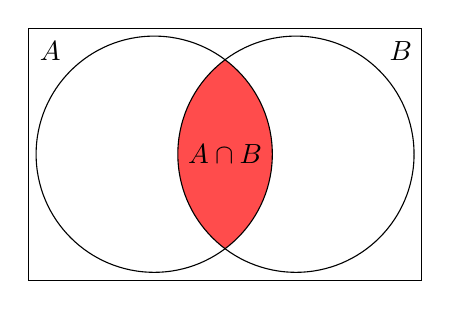
\begin{tikzpicture}
    \draw (-1.6,-1.6) rectangle (3.4,1.6);
    % Set A
    \node[circle,minimum size = 3cm,label={135:$A$}] (A) at (0,0) {}; %"minimum size" is the diameter. "label={135:$A$}" positions texts $A$ at 135 degrees of the circle. 
    
    % Set B
    \node[circle,minimum size = 3cm,label={45:$B$}] (B) at (1.8,0) {};
    %"minimum size" is the radius. "label={45:$B$}" positions texts $B$ at 45 degrees of the circle. 

    % Intersection
    \begin{scope}
        \clip (0,0) circle(1.5cm);
        \clip (1.8,0) circle(1.5cm);
        \fill[red!70](0,0) circle(1.5cm);
    \end{scope}
    
    % Circles outline
    \draw (0,0) circle(1.5cm);
    \draw (1.8,0) circle(1.5cm);
    
    % Set intersection label
    \node at (0.9,0) {$A\cap B$};
    
\end{tikzpicture}
\end{document}